\section*{Problem 1: Forward Kinematics} \label{Sec: Problem 1: Forward Kinematics}


	The first problem encountered is to describe both the position of the tool, and the locations
	A and B (and most likely the entire surface $S$) with respect to a common coordinate
	system. The reason why we want to do this to express mathematically where the robot is, with regards to the surface.
	In Chapter 2 we will give some background on representations of coordinate systems and how these coordinate systems relate to each other.\\

	\begin{figure}[H]
		\centering
		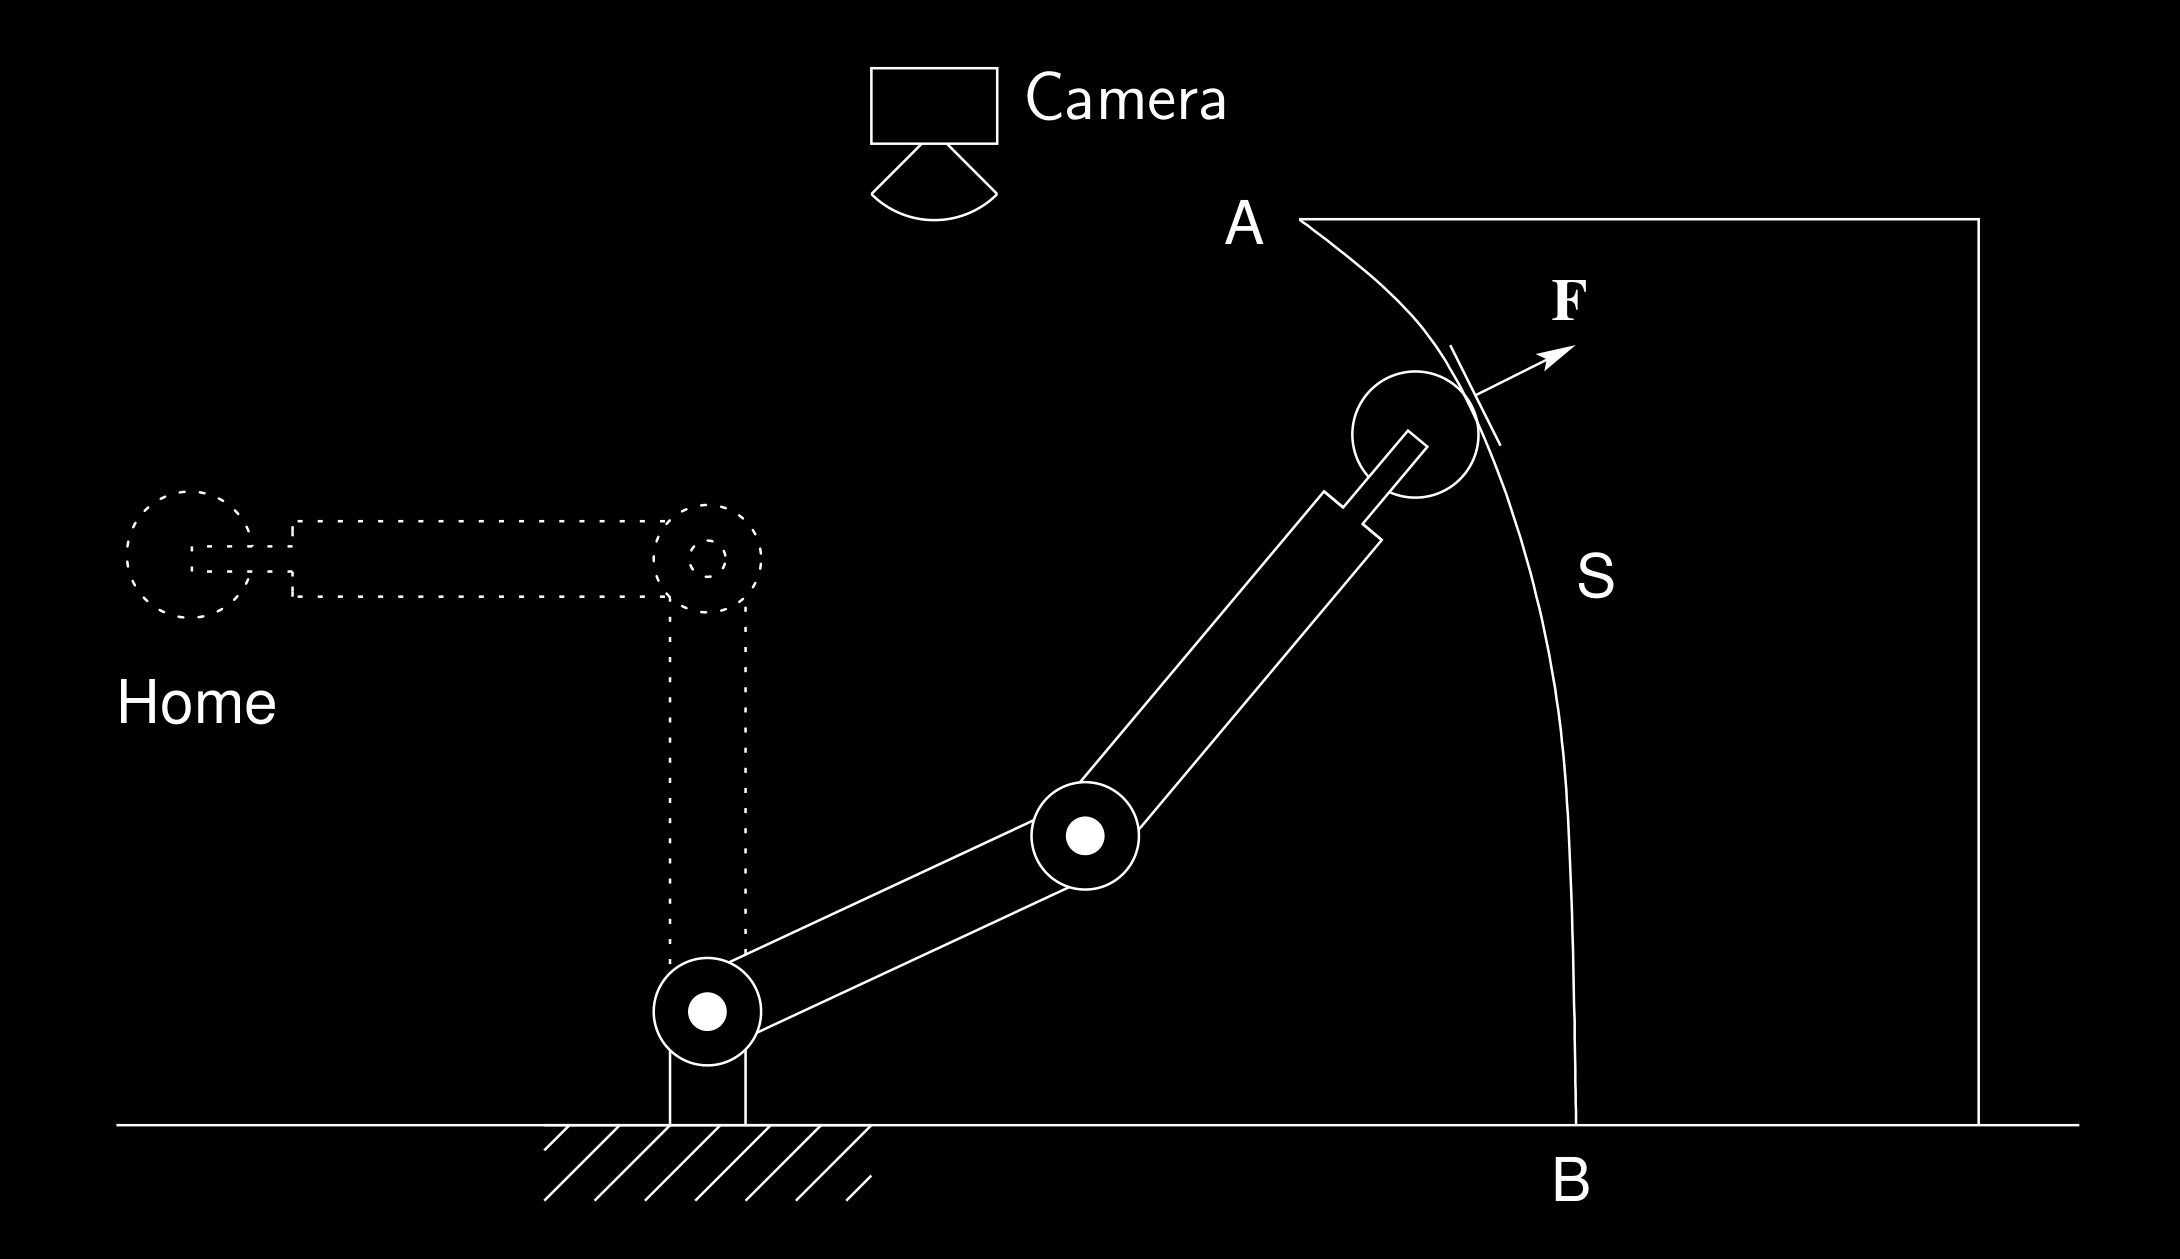
\includegraphics[width=0.8\textwidth]{img/Figure1_24.png}
		\caption{Two-link planar robot example}
		\label{fig:Figure1_24}
	\end{figure}

	Typically, the manipulator will be able to sense its own position in some manner using internal sensors, often position encoders, but sometimes resolvers, especially for revolute joints. In the case of Figure \ref{fig:Figure1_25}, the sensors for measuring degrees of rotation are located in the center of joints 1 and 2, so that they can measure directly the joint angles $\theta_1$ and $\theta_2$. Therefore, we also need to express the positions $A$ and $B$ in
	terms of these joint angles. This leads to the \textbf{Forward Kinematics problem}, which is the cornerstone of understanding robotics.
	Rephrased, we can say that \textbf{Forward Kinematics} is a mathematical problem where we want to determine the position and
	orientation of the end-effector or tool in terms of the robots joint variables and link lenghts. We will study this topic thoroughly later on in	Chapter 3.\\

	It is customary to establish a fixed coordinate system, called the \textbf{world} or \textbf{base} frame
	to which all objects including the manipulator are referenced. In real world applications of robots, these frames rarely coincide, but for simplification purposes they can sometimes be the same. The \textbf{base} frame should always be located at the robots base, this convention is however not always followed. In our case we follow the convention and establish the base coordinate frame denoted $o_{0}x_{0}y_{0}$ at the base of the robot. Furthermore, we will establish the coordinate system $o_{1}x_{1}y_{1}$ at the center of joint 2, and the coordinate system $o_{2}x_{2}y_{2}$ at the tip of the robot where it's end-effector is located. This is shown below in Figure \ref{fig:Figure1_25}.

	\begin{figure}[H]
		\centering
		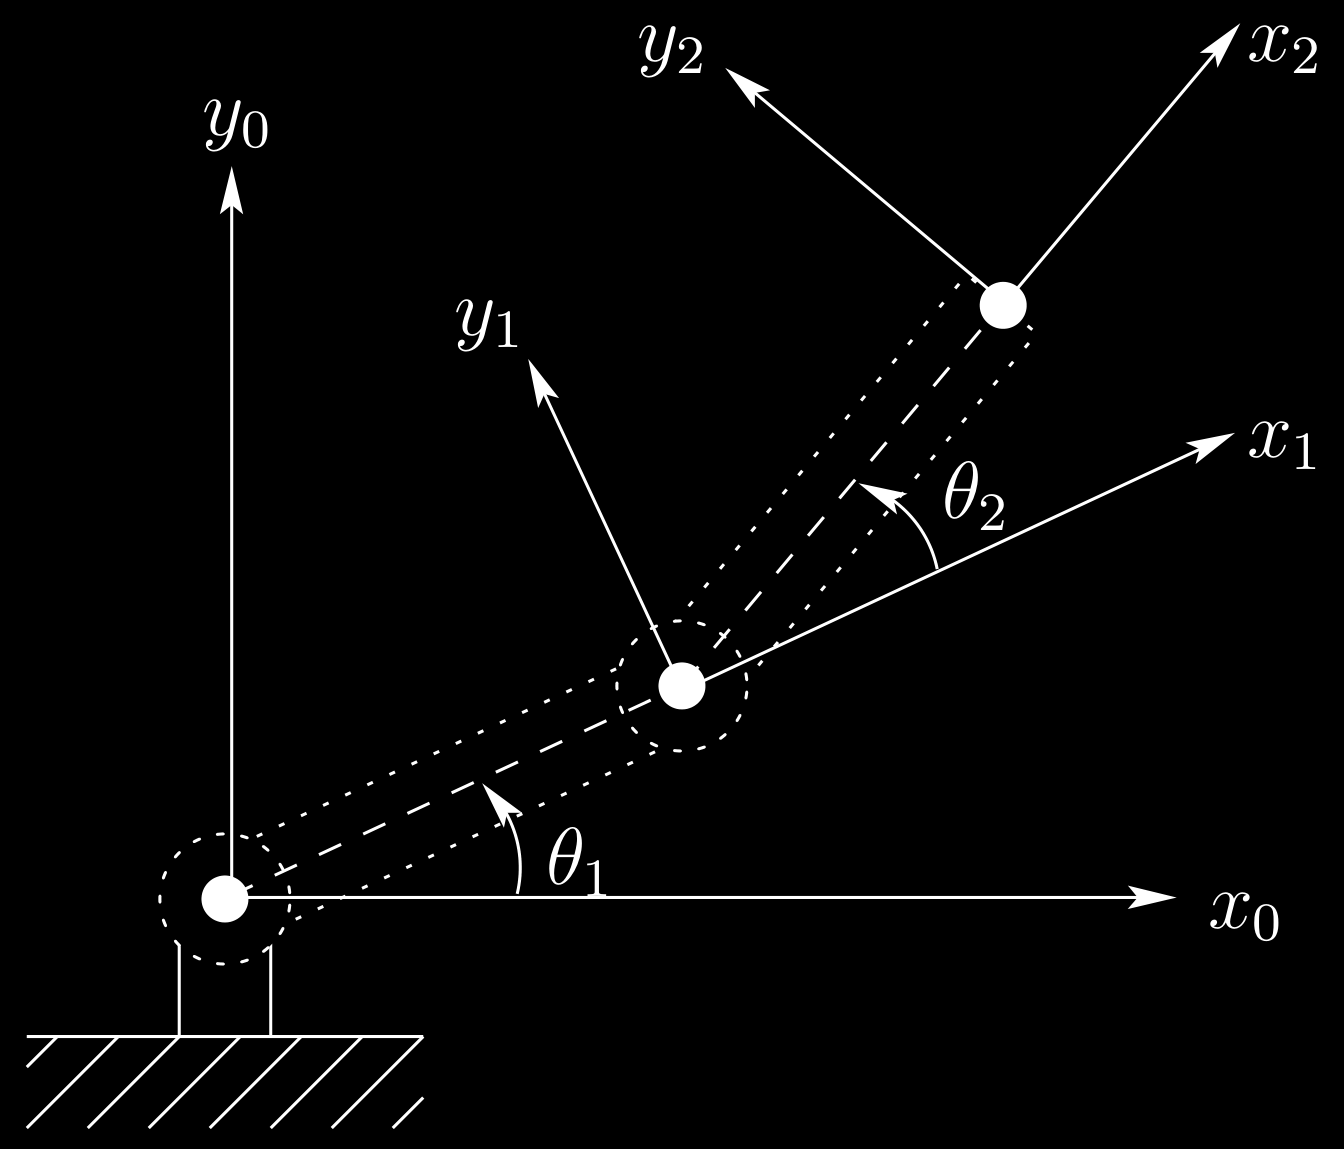
\includegraphics[width=1\textwidth]{img/Figure1_25.png}
		\caption{Coordinate frames for two-link planar robot}
		\label{fig:Figure1_25}
	\end{figure}

	The somewhat mystical notation $o_{0}x_{0}y_{0}$ is usually written short as $o_{0}$. By adding $x_{0}y_{0}$ we intend to specify that the coordinate system $o_{0}$ is spanned by the vectors $x_{0}$ and $y_{0}$.\\ Why do we need that, why two vectors, should we not specify three, or maybe four, just to be sure? Well, the robot in Figure \ref{fig:Figure1_25} lives in a two-dimensional space, thus it can not move in a third direction, meaning we only need two vectors to mathematically describe the robots action in the world. If you are not familiar with vectors, just imagine these vectors as arrows of infinite length making up the whole coordinate system.\\

	\newpage

	Let now the tool of the robot be located at the origin of $o_2$, and let $(x,y)$ be the coordinates of the tool, expressed in the \textbf{base} coordinate frame. This means that $x$ represent a distance between the origin of $o_0$ and some random place on the $x_{0}$ vector, and $y$ represent the position along the $y_{0}$ vector. We see now that since we have specified the $x_{0}$ and $y_{0}$ vectors, we know in which direction $x$ and $y$ are going. Thus the specification of $x_{0}$ and $y_{0}$ becomes significant. Moreover, with some basic trigonometry, we can express the coordinates $(x,y)$ by just drawing some lines:

	\begin{figure}[H]
		\centering
		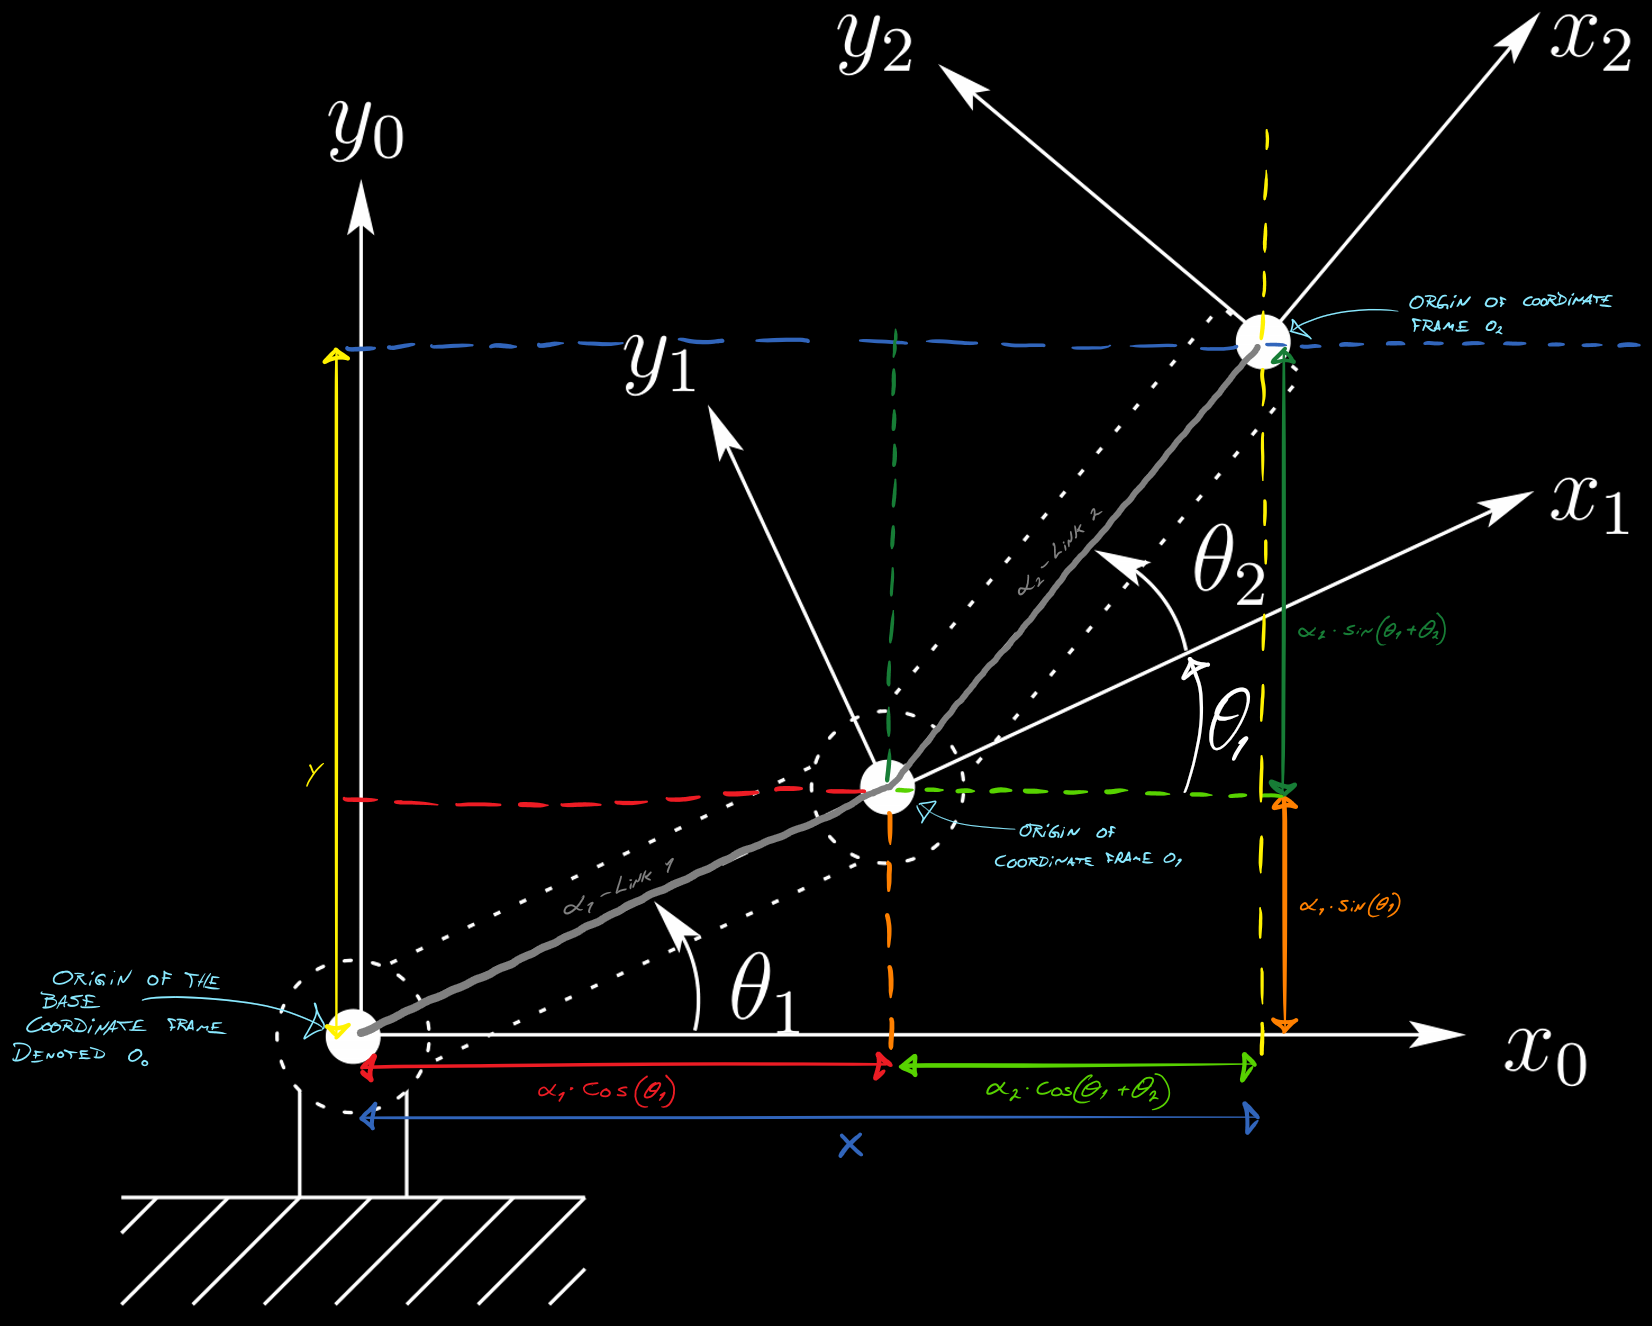
\includegraphics[width=1\textwidth]{img/Figure1_25_drawing.png}
		\caption{Coordinate frames for two-link planar robot}
		\label{fig:Figure1_25_drawing}
	\end{figure}

	Hence we see that when $\alpha_1$ and $\alpha_2$ are the lengths of the two links, respectively, we get

	\begin{equation} \label{eq:positionX}
		x = \alpha_{1}\cos{\theta_1} + \alpha_{2}\cos(\theta_{1} + \theta_{2})
	\end{equation}

	\begin{equation} \label{eq:positionY}
		y = \alpha_{1}\sin{\theta_1} + \alpha_{2}\sin(\theta_{1} + \theta_{2})
	\end{equation}


	If you don't know what $\cos(x)$ and $\sin(x)$ are, don't despair. Just think of them as functions that takes in a number (which could be any number on the real number line) and outputs a value which lies in the continuous interval of real numbers between $-1$ and $1$.\\
	I.e.\\ $\cos(\frac{\pi}{2}) = 0$, $cos(\pi) = -1$, $cos(1048576\pi) = 1$, $sin(\frac{\pi}{2}) = 1$, $sin(\frac{3\pi}{2}) = -1$, $sin(1048576\pi) = 0$.\\

	We have now found the position of the end-effector. Thus, it remains to express how the coordinate system $o_2$ which represent the orientation of the tool, has rotated with respect to $o_0$.
	We do this by arranging the representation in a rather different way called a matrix. A matrix is a collection of numbers arranged into a fixed number of rows and columns, which is convenient for us, since the tool coordinate frame $o_2$ has two vectors $x_{2}$ and $y_{2}$ rotated with respect to two other vectors $x_{0}$ and $y_{0}$ (which composes $o_0$). Thus we will need four numbers to represent our rotation.\\


	Let now

	\begin{itemize}

		\item $\gamma_1$ represent the rotation of $x_{2}$ with respect to the $x$ axis of the base frame, namely $x_{0}$
		\item $\gamma_2$ represent the rotation of $x_{2}$ with respect to the $y$ axis of the base frame, namely $y_{0}$
		\item $\gamma_3$ represent the rotation of $y_{2}$ with respect to the $x$ axis of the base frame, namely $x_{0}$
		\item $\gamma_4$ represent the rotation of $y_{2}$ with respect to the $y$ axis of the base frame, namely $y_{0}$

	\end{itemize}

	Then


	\begin{equation} \label{eq:orientation}
		\begin{bmatrix}
			\gamma_1 & \gamma_3 \\
			\gamma_2 & \gamma_4
		\end{bmatrix}
		=
		\begin{bmatrix}
			\cos(\theta_{1} + \theta_{2}) & -\sin(\theta_{1} + \theta_{2}) \\
			\sin(\theta_{1} + \theta_{2}) & \cos(\theta_{1} + \theta_{2})
		\end{bmatrix}
	\end{equation}

	And we now have our orientation representation. To summarize, the equations (\ref{eq:positionX}), (\ref{eq:positionY}) and (\ref{eq:orientation}) represent the robots position and orientation in the two-dimensional world it is operating within, and hence these are the \textbf{Forward Kinematics equations}.
	For a six degree-of-freedom robot these equations are quite complex and cannot be written down as easily as for the two-link manipulator. The general procedure that we discuss in Chapter 3 establishes coordinate frames at each joint and allows one to transform systematically among these frames using matrix transformations. The procedure that we use is referred to as the \textbf{Denavit-Hartenberg convention}.
